\documentclass[tikz,border=10pt]{standalone}

% Basis mismatch: a single d-bit AND is 1 Möbius coefficient
% but 2^d Fourier (parity) coefficients. Shown for d = 3.

\usepackage{tikz}
\usetikzlibrary{arrows.meta,calc}
\usepackage{amsmath,amssymb}
\usepackage{xcolor}

\definecolor{mobiuscolor}{RGB}{0,100,200}
\definecolor{fouriercolor}{RGB}{200,50,50}

\begin{document}
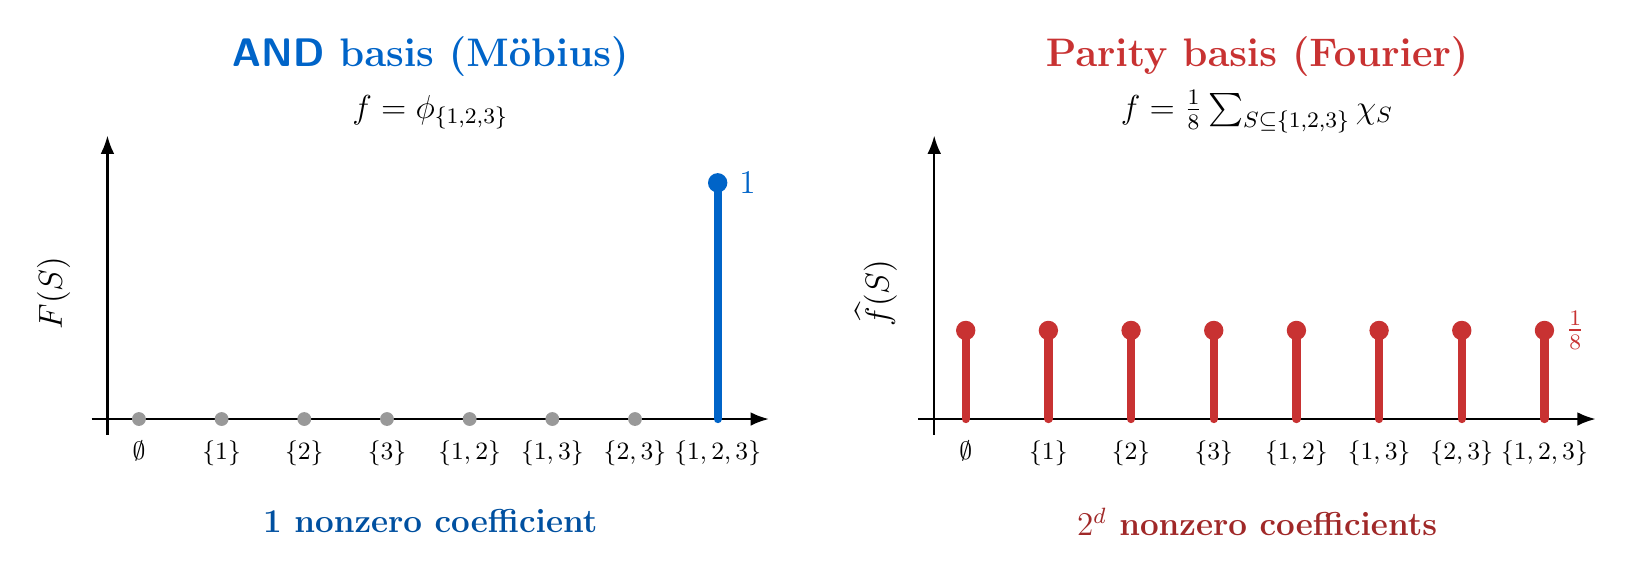
\begin{tikzpicture}[
  every node/.append style={font=\large},
  stem/.style={line width=3pt, line cap=round},
]

% ---------- common data ----------
\def\labels{{"$\emptyset$","$\{1\}$","$\{2\}$","$\{3\}$","$\{1,2\}$","$\{1,3\}$","$\{2,3\}$","$\{1,2,3\}$"}}
\def\dx{1.05}   % horizontal spacing between stems
\def\ymax{3.0}  % height of unit coefficient

% ---------- left panel: Mobius (AND basis) ----------
\begin{scope}[shift={(0,0)}]
  \node[font=\Large\bfseries, mobiuscolor] at (3.7, 4.6) {\textsf{AND} basis (M\"obius)};
  \node[font=\large] at (3.7, 3.9) {$f = \phi_{\{1,2,3\}}$};

  % axes
  \draw[-Latex, thick] (-0.6, 0) -- (8.0, 0);
  \draw[-Latex, thick] (-0.4, -0.2) -- (-0.4, 3.6);
  \node[rotate=90, anchor=south] at (-0.75, 1.6) {$F(S)$};

  % stems (all zero except {1,2,3})
  \foreach \i in {0,...,6} {
    \fill[black!40] ({\i*\dx}, 0) circle (2.5pt);
  }
  \draw[stem, mobiuscolor] ({7*\dx}, 0) -- ({7*\dx}, \ymax);
  \fill[mobiuscolor] ({7*\dx}, \ymax) circle (3.5pt);
  \node[anchor=west, mobiuscolor] at ({7*\dx+0.15}, \ymax) {$1$};

  % x labels
  \foreach \i in {0,...,7} {
    \pgfmathsetmacro{\lab}{\labels[\i]}
    \node[anchor=north, font=\small, rotate=0] at ({\i*\dx}, -0.15) {\lab};
  }

  \node[font=\large, mobiuscolor!80!black, align=center] at (3.7, -1.3)
    {\textbf{1 nonzero coefficient}};
\end{scope}

% ---------- right panel: Fourier (parity basis) ----------
\begin{scope}[shift={(10.5,0)}]
  \node[font=\Large\bfseries, fouriercolor] at (3.7, 4.6) {Parity basis (Fourier)};
  \node[font=\large] at (3.7, 3.9) {$f = \tfrac{1}{8}\sum_{S \subseteq \{1,2,3\}} \chi_S$};

  % axes
  \draw[-Latex, thick] (-0.6, 0) -- (8.0, 0);
  \draw[-Latex, thick] (-0.4, -0.2) -- (-0.4, 3.6);
  \node[rotate=90, anchor=south] at (-0.75, 1.6) {$\widehat{f}(S)$};

  % stems: all 2^d subsets get height 1/8
  \foreach \i in {0,...,7} {
    \draw[stem, fouriercolor] ({\i*\dx}, 0) -- ({\i*\dx}, {\ymax/8*3});
    \fill[fouriercolor] ({\i*\dx}, {\ymax/8*3}) circle (3.5pt);
  }
  \node[anchor=west, fouriercolor] at ({7*\dx+0.15}, {\ymax/8*3}) {$\tfrac{1}{8}$};

  % x labels
  \foreach \i in {0,...,7} {
    \pgfmathsetmacro{\lab}{\labels[\i]}
    \node[anchor=north, font=\small] at ({\i*\dx}, -0.15) {\lab};
  }

  \node[font=\large, fouriercolor!80!black, align=center] at (3.7, -1.3)
    {\textbf{$2^d$ nonzero coefficients}};
\end{scope}

\end{tikzpicture}
\end{document}
